\documentclass[conference , 12pt]{IEEEtran}
\IEEEoverridecommandlockouts
\usepackage{cite}
\usepackage{amsmath,amssymb,amsfonts}
\usepackage[margin=0.8in , pass,paperwidth=8.5in,paperheight=11in]{geometry}
\usepackage{algorithmic}
\usepackage{graphicx}
\usepackage{textcomp}
\usepackage{adjustbox}
\usepackage{subcaption}
\usepackage{enumitem}
\usepackage{multirow}
\usepackage{bbding,enumitem}
\usepackage{authblk}
\usepackage{booktabs}
\usepackage{xcolor}
\usepackage{url}
\usepackage{times}
\usepackage{titlesec} 
\usepackage{tocloft}

\renewcommand{\thesection}{\arabic{section}}
\renewcommand{\thesubsection}{\thesection.\arabic{subsection}}
\renewcommand{\thesubsubsection}{\thesubsection.\arabic{subsubsection}}

% Define subsubsubsection with numbering (1.1.1.1)
\titleformat{\paragraph}
  {\normalfont\normalsize\itshape}{\theparagraph}{1em}{}

\renewcommand{\theparagraph}{\thesubsubsection.\arabic{paragraph}}
\setcounter{secnumdepth}{4}  % Allow numbering for \paragraph
\setcounter{tocdepth}{4}     % Allow \paragraph to appear in ToC


\makeatletter
\def\@seccntformat#1{\csname the#1\endcsname\quad}
\makeatother

\usepackage{fancyhdr}
\pagestyle{fancy}

\begin{document}
\onecolumn

\lhead{{Contents}}

\tableofcontents
\newpage

\twocolumn

\fancyhf{}
\lhead{\nouppercase {\leftmark}}
\rhead{\thepage}
\fancyfoot[L]{\hspace*{-1.9cm}\raisebox{-1.3cm}{
\includegraphics[width=\paperwidth,height=1.9cm]{1Images/Footer.png}}} % Footer

\section{Abstract}

\begin{abstract}
    Hi, this is the abstract O\_\_\O!
\end{abstract}

\newpage

\section{Design Evolution}


\newpage


\section{Design \& Manufacturing Process}
\subsection{Mechanical}
\subsection{Probably something mechanical}
YOU WOULD NOT BELIEVE IT. but, it's probably something mechanical.

\subsubsection{Mechanical Design}



\vspace{5cm} 
\subsection{Electrical}
\subsection{Probably something electrical}

yeah, probably something electrical.

\vspace{5cm}
\subsection{Software}
<<<<<<< Updated upstream
\subsubsection{Kinematics}
The Kamikaze's movement underwater may be one of the most important aspects of
the design. We had to ensure stability, maneuverability, and speed. We achieved
this by focusing on two main aspects:
\begin{itemize}
        
    \item \textbf{Thrusters Configuration:} We employed a seventh thruster this year to
        improve the robot's maneuverability. With the current vectored thrusters
        configuration and this new thruster, we can achieve motion in 6 degrees of freedom.
        This novel configuration may be the first of its kind to allow for such a wide range of motion while only using 7 thrusters.

        \item \textbf{PID Control:} We have implemented PID controllers for all critical movement axes, allowing for
        precise control over the robot's movement and ensures that it remains stable in the water. We implemented an FFT (Fast Fourier Transform)
        based auto-tuning algorithm to tune the PID parameters, as this is our first year using the new Vehicle. We also supplemented the algorithm with a live
        plotting feature, shown in figure \ref{fig:pid_live},
         to allow for manual adjustments to the PID parameters.
\end{itemize}
\begin{figure}[h]
    \centering
    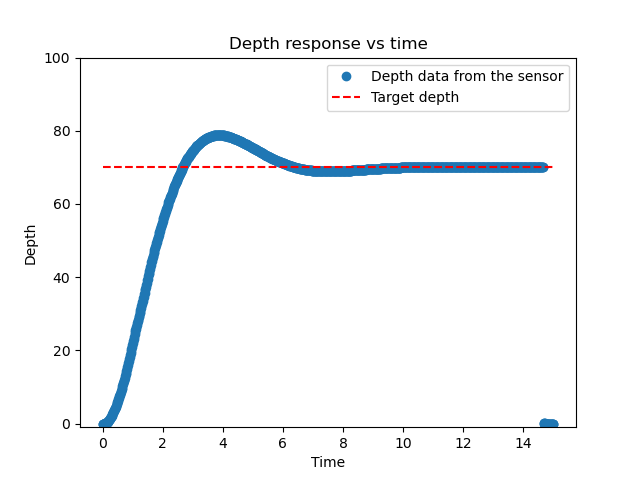
\includegraphics[width=0.5\textwidth]{Sections/3Design&Manufacturing/tex/Software/images/Pid.png}
    \caption{Live Plotting of PID Parameters}
    \label{fig:pid_live}
\end{figure}

\subsection{Open Sourcing the Kamikaze}
We have all of our working code available on our GitHub repository. A lot of effort
was made this year to maintain, document, and clean up the code, making it easier
for future teams to understand and build upon. We believe that this is a crucial
step in the development of the Kamikaze, as it allows for a more collaborative
environment and ensures that the knowledge gained from each year is not lost. 

=======
\section{Communication Architecture}
The ROV's communication architecture which is illustrated in Figure 1 can be divided into two parts: the top side control unit and the ROV unit.

\begin{figure}[ht]
    \centering
    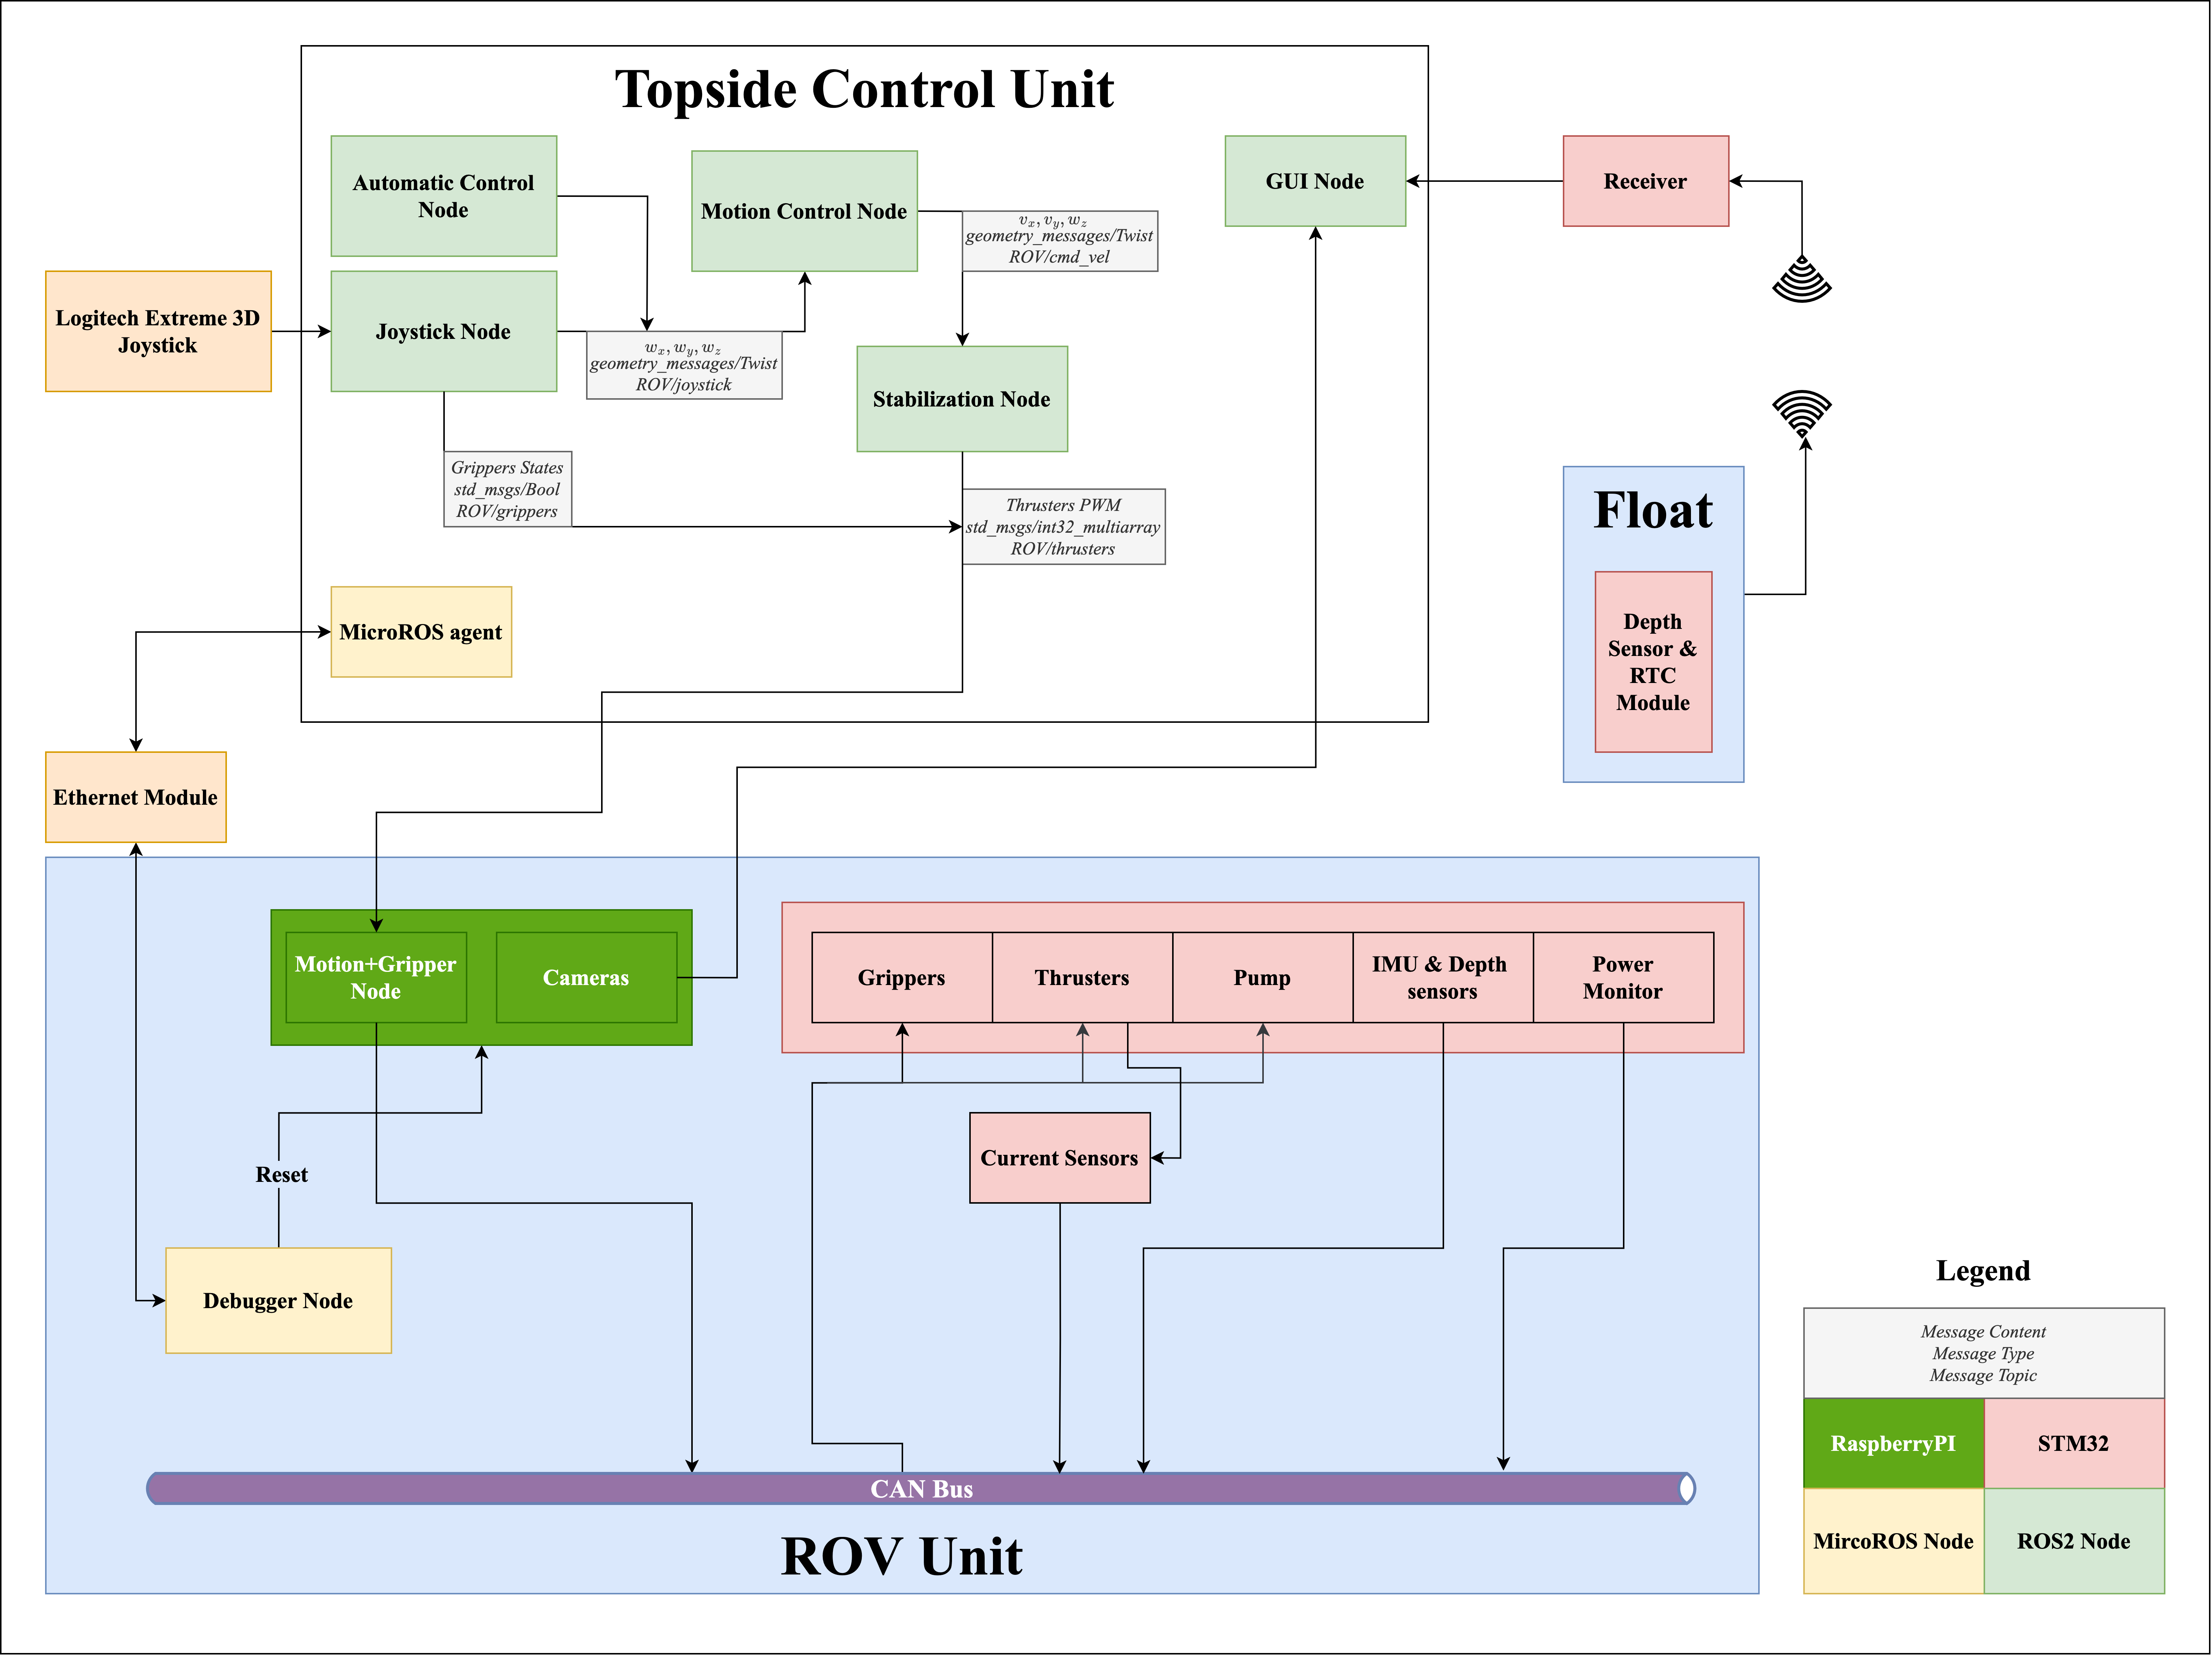
\includegraphics[width=1\linewidth]{rov_architecture_2.png}
    \caption{Communication architecture}
\end{figure}

\subsection{System Evolution and Communication Backbone}

In last year's architecture, we utilized ROS 1 as the main framework for communication between the control unit and the ROV's micro-controllers. 

Communication with MCUs was handled through \texttt{rosserial}, which introduced a critical limitation: the presence of a single point of failure—the ROS Master. Any instability or failure in the master would cause the entire system to halt, making it unreliable in underwater environments where robustness is essential.

\vspace{0.5em}
This year, we have transitioned fully to ROS 2, eliminating the dependency on a centralized master. Communication between the topside control unit and the ROV unit is now handled using ROS2 \& CAN communication, which is more reliable, scalable, and real-time capable.
\vspace{0.5em}


In parallel, we’ve integrated \texttt{micro-ROS} to run a debugger node on the ROV side. This node communicates with the topside unit via an Ethernet module, acting as a backup communication path. In the event of failure of our SBC—the Raspberry Pi, this channel ensures continued monitoring of the entire system's vitals which greatly facilitates debugging in case of a problem with our system.

\vspace{0.5em}
This upgraded architecture enhances reduces the risk of total system failure, making it far more suitable for mission-critical underwater operations and industrial applications.

\subsection{Topside Control Unit}
The topside control unit hosts the nodes and agents that work above water which includes:
\begin{itemize}
    \item Joystick Node
    \item Automatic Control Node
    \item Stabilization Node
    \item Motion Control Node 
    \item GUI Node
    \item Micro-ROS agent
\end{itemize}
Data is received from the following streams:
\begin{itemize}
    \item Camera feed from the ZED camera as well as the side-assisting cameras
    \item Readings from sensors which includes an IMU sensor and a depth sensor
    \item Readings from the joystick
    \item Receiver from the Float unit
\end{itemize}
The joystick node is interfaced with the Logitech Extreme 3D Pro Joystick, capturing signals and converting them into ROS messages, which then are sent over to the motion control node in order to order to convert these signals to motion vectors and gripper operations. 

For autonomous tasks, the automatic control node is pivotal. It receives commands from the joystick and autonomously sends out commands to the motion control node.

The motion control node converts the received messages into motion vectors that are then sent to the stabilization node.

The stabilization node is used to maintain the operational stability of the ROV by applying various PID controllers to counter any disturbances.

The GUI node acts as the pilot's interface, displaying camera feeds for navigation as well as displaying the ROV's vitals.

Vitals include: 
\begin{itemize}
    \item IMU readings
    \item Depth readings from both the ROV unit and the Float unit
    \item Thrusters PWM values
\end{itemize}

\subsection{ROV Unit}
The ROV unit is where a lot of the heavy lifting happens, it executes commands received from the topside control unit, streams cameras and hosts the debugger node.

The ROV unit has a Raspberry Pi 5 that's responsible for streaming cameras to the GUI node as well as it hosts a ROS 2 node that is responsible for receiving the commands from the stabilization node.

Connected to the Raspberry Pi 5 is the CAN bus where it receives data from sensors such as current sensors, a depth sensor, an IMU and the power monitor.
That are then published to both the topside control unit as well as the debugger node.

\subsection{Float Unit}
The float unit hosts a depth senor that transmits it's readings using an NRF transceiver module and an RTC (Real-time Clock) to the receiver which are then displayed on the GUI in the topside control unit.
>>>>>>> Stashed changes

\newpage


\section{Mission-Specific auxiliary tools}


\newpage

\section{Testing \& Validation}


\newpage

\section{Logistics}


\newpage

\section{Budget \& Accounting}


\newpage
\end{document}